\documentclass[12pt]{article}

\usepackage[pdftex]{graphicx}
\usepackage{amsmath}
\usepackage{enumitem}


\newcommand\tab[1][1cm]{\hspace*{#1}}
\newcommand{\HRule}{\rule{\linewidth}{0.5mm}}

% Margins
\topmargin=-0.45in
\evensidemargin=0in
\oddsidemargin=0in
\textwidth=6.5in
\textheight=9.0in
\headsep=0.25in
\title{ COMS 474\\Homework 3 }
\author{ Haadi Majeed }
\date{Spring 2022}

\usepackage{cancel}
\usepackage[margin=4cm]{geometry}
\usepackage[hidelinks]{hyperref}
\usepackage{fancyhdr}
\pagestyle{fancy}
\fancyhead{}
\fancyfoot{}
\lhead{COMS 474}
\chead{Haadi Majeed}
\rhead{Page \thepage}

\begin{document}
\maketitle
\pagebreak

% Optional TOC
% \tableofcontents
% \pagebreak
\section*{Problem 1}
 [26 points total ]\\
For the following, you will look at how the underlying $f(X)$ and the number of samples play a role in the occurrence and extent of both under-fitting and over-fitting. You will use the Jupyter notebook posted on canvas along with these directions. You should only need to modify two variables in the last code block, setting $f\_type$ to ‘linear’ or ‘sinusoidal’ and setting $n\_samples$ to 15 or 1000.
\\\\
Recall that there are many factors that affect how well a fitted model will perform on future data, including the class of models we are using for fitting (here polynomials), the underlying trend $f(X)$, the noise (here additive Gaussian), and the number of samples.
\\\\
\textbf{\underline{Additional Notes}}
\begin{itemize}
    \item The results are random, since the data set itself is random.
    \item You are encouraged to re-run the code for each setting a few times to gain some insight into the variability of the results. We will explore this issue in more depth later on.
    \item The $Y$ axis for the MSE figure does not have fixed limits. Pay attention to the range of the MSE values as you compare plots.
\end{itemize}

\begin{enumerate}[label=(\alph*)]
    \item Using a sinusoidal $f(X)$ and noise standard deviation $\sigma = 5$, plot the estimated models and the MSE curves for
          \begin{enumerate}[label=(\roman*)]
              \item $n = 15$ samples
              \item $ n = 1000$ samples
          \end{enumerate}
          Using those four plots, comment on whether under-fitting and/or over-fitting occur and the extent to which they do for each of i. and ii. Then discuss how the number of samples affects the result (eg similarities and differences between i. and ii.)\\
          \begin{center}
              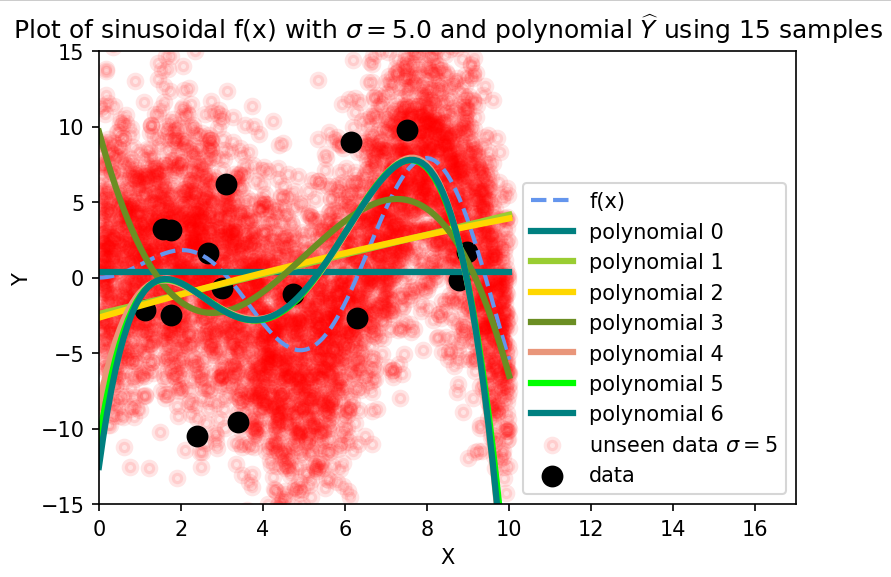
\includegraphics[width=1\textwidth]{sinosodial-15.png}
              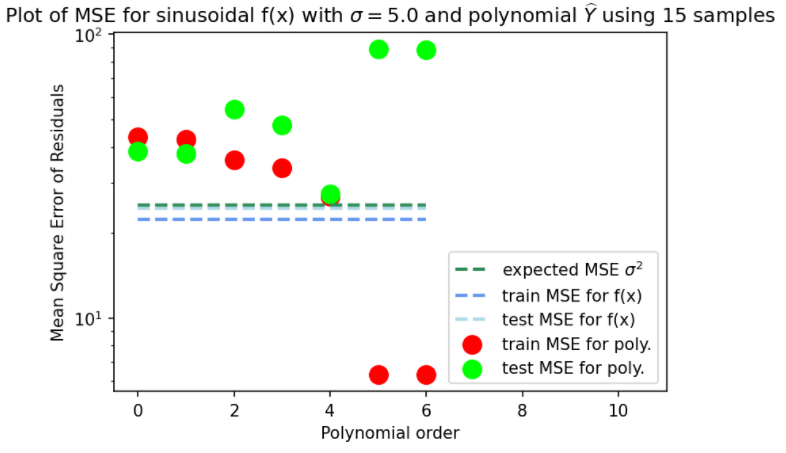
\includegraphics[width=1\textwidth]{sinosodial-MSE-15.png}
              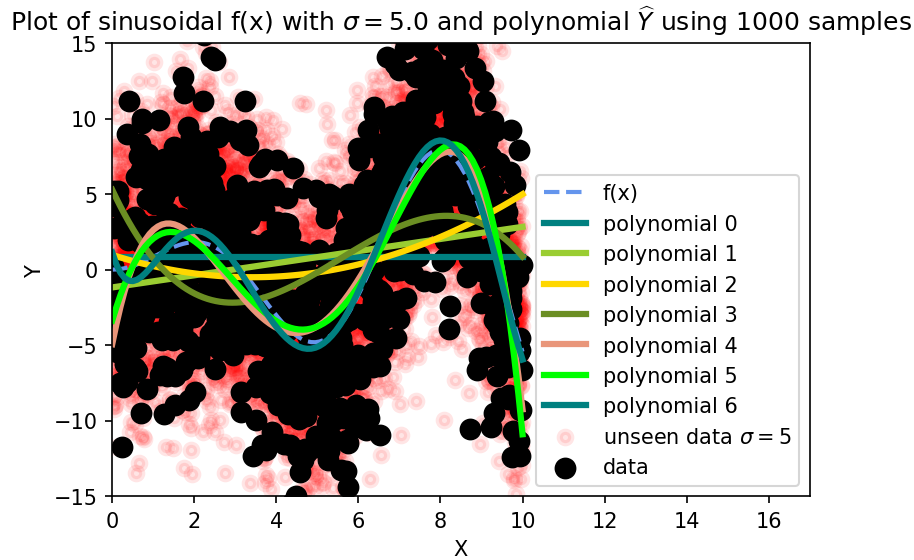
\includegraphics[width=1\textwidth]{sinosodial-1000.png}
              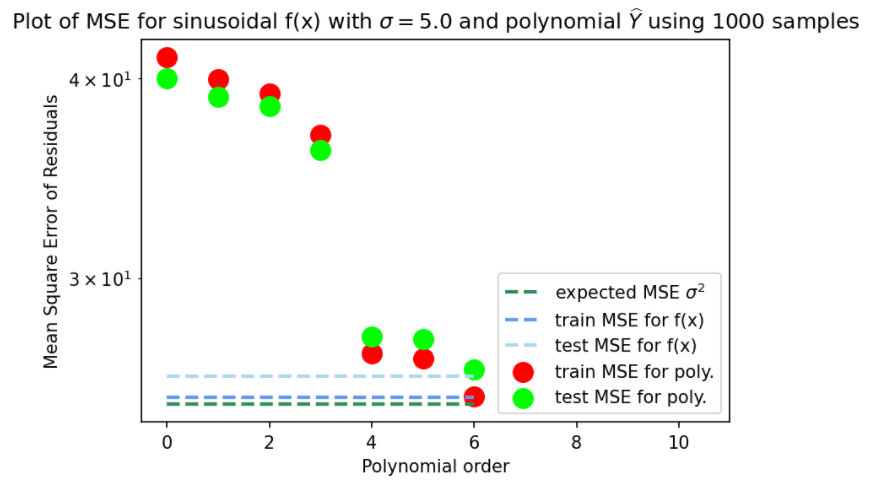
\includegraphics[width=1\textwidth]{sinosodial-MSE-1000.png}
          \end{center}
    \item Repeat (a) with a linear $f(X)$.
          \begin{center}
              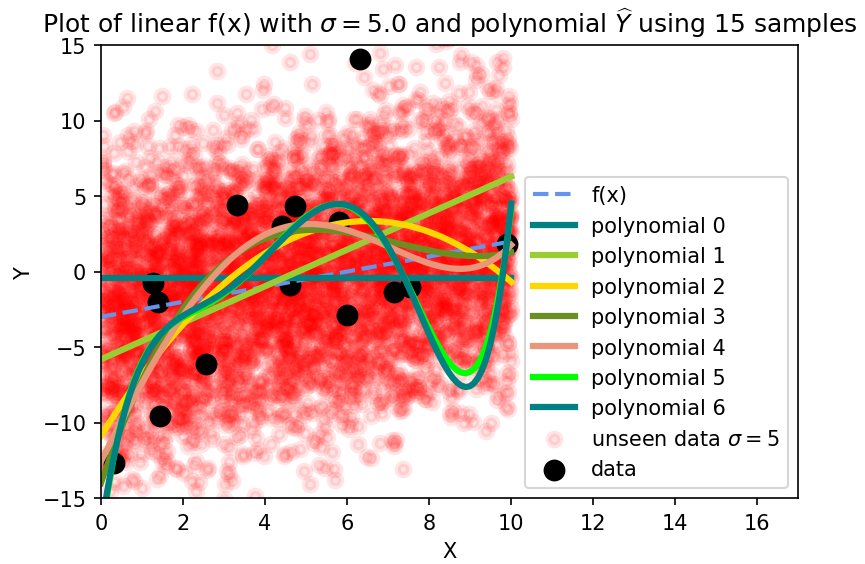
\includegraphics[width=1\textwidth]{linear-15.png}
              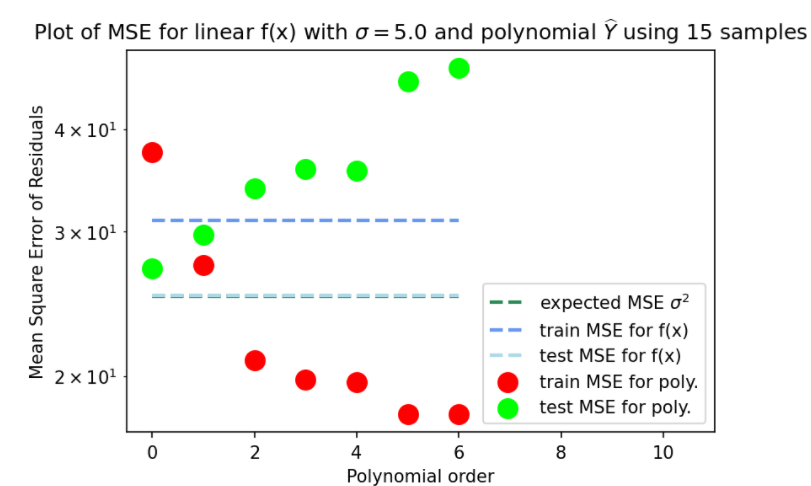
\includegraphics[width=1\textwidth]{linear-MSE-15.png}
              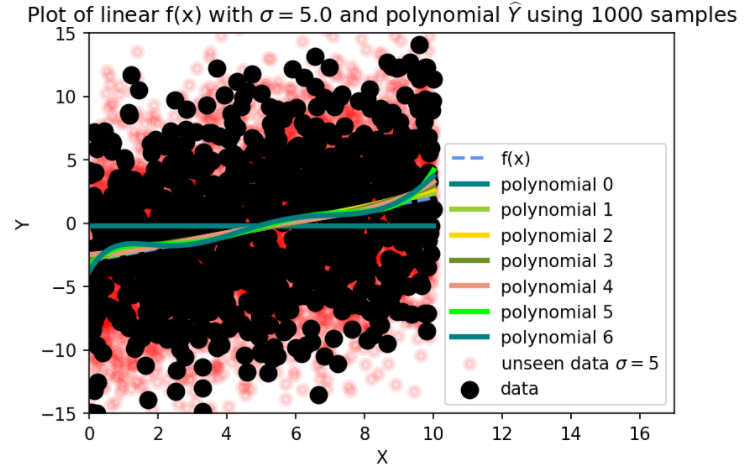
\includegraphics[width=1\textwidth]{linear-1000.png}
              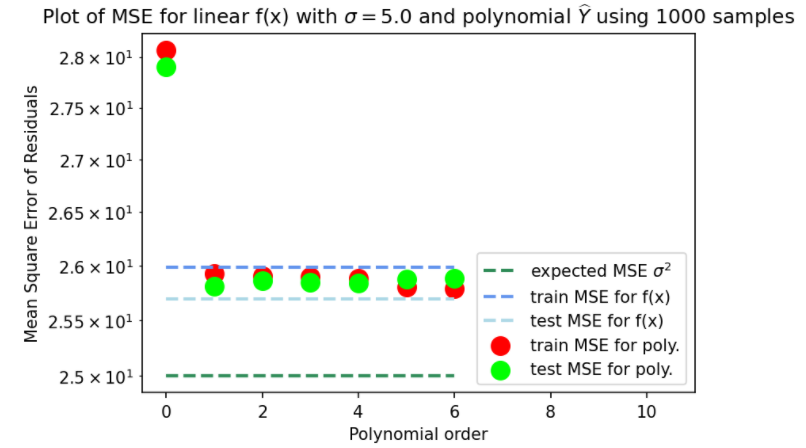
\includegraphics[width=1\textwidth]{linear-MSE-1000.png}
          \end{center}
    \item Now discuss similarities and differences between the results of (a) and (b), given that the main difference was $f(X)$ (which for (a) was not only non-linear in $X$ but also not in the model class we were fitting with, while for (b) it was linear and in the model class).
\end{enumerate}
%--/Paper--

\end{document}